\section{\edited{Sensitivity grid}}\label{app:sensitivity}
{\color{red}
Figure~\ref{fig:sensitivity-scores} shows the mean score changes from the
same-seed primary specification over five seeds.
Figure~\ref{fig:sensitivity-aggregate} reports percentage changes in
aggregate deviation. M1 changes concern tail weighting of standardized
marginal returns; M4 changes concern volatility conditioning and tail shape.
The full numerical settings, seed-level results, coverage diagnostics,
and summary tables are recorded with the repository's sensitivity results.
Ranges across seeds are numerical diagnostics, not corpus confidence intervals.
}
\begin{table}[htbp]
\centering
\color{red}
\caption{Ranges of paired changes from the same-seed primary across the tested alternatives and five seeds. M1 and M4 entries are score differences; aggregate entries are percentage changes in $G_{\mathrm{dev}}$. These minima and maxima are not confidence intervals.}
\label{tab:sensitivity-ranges}
\small
\begin{tabular}{@{}lccc@{}}
\toprule
Generator & M1 change & M4 change & $G_{\mathrm{dev}}$ change (\%) \\
\midrule
AIL & $[-0.0452, 0.0144]$ & $[-0.0378, 0.0181]$ & $[-1.80, 5.08]$ \\
GBM & $[-0.0008, 0.0009]$ & $[-0.0086, 0.0072]$ & $[-4.45, 6.74]$ \\
MSV & $[-0.0140, 0.0058]$ & $[-0.0240, 0.0149]$ & $[-4.08, 8.56]$ \\
SBBTS & $[-0.0006, 0.0017]$ & $[-0.0121, 0.0168]$ & $[-3.75, 3.00]$ \\
\bottomrule
\end{tabular}
\end{table}

\begin{figure}[htbp]
\centering
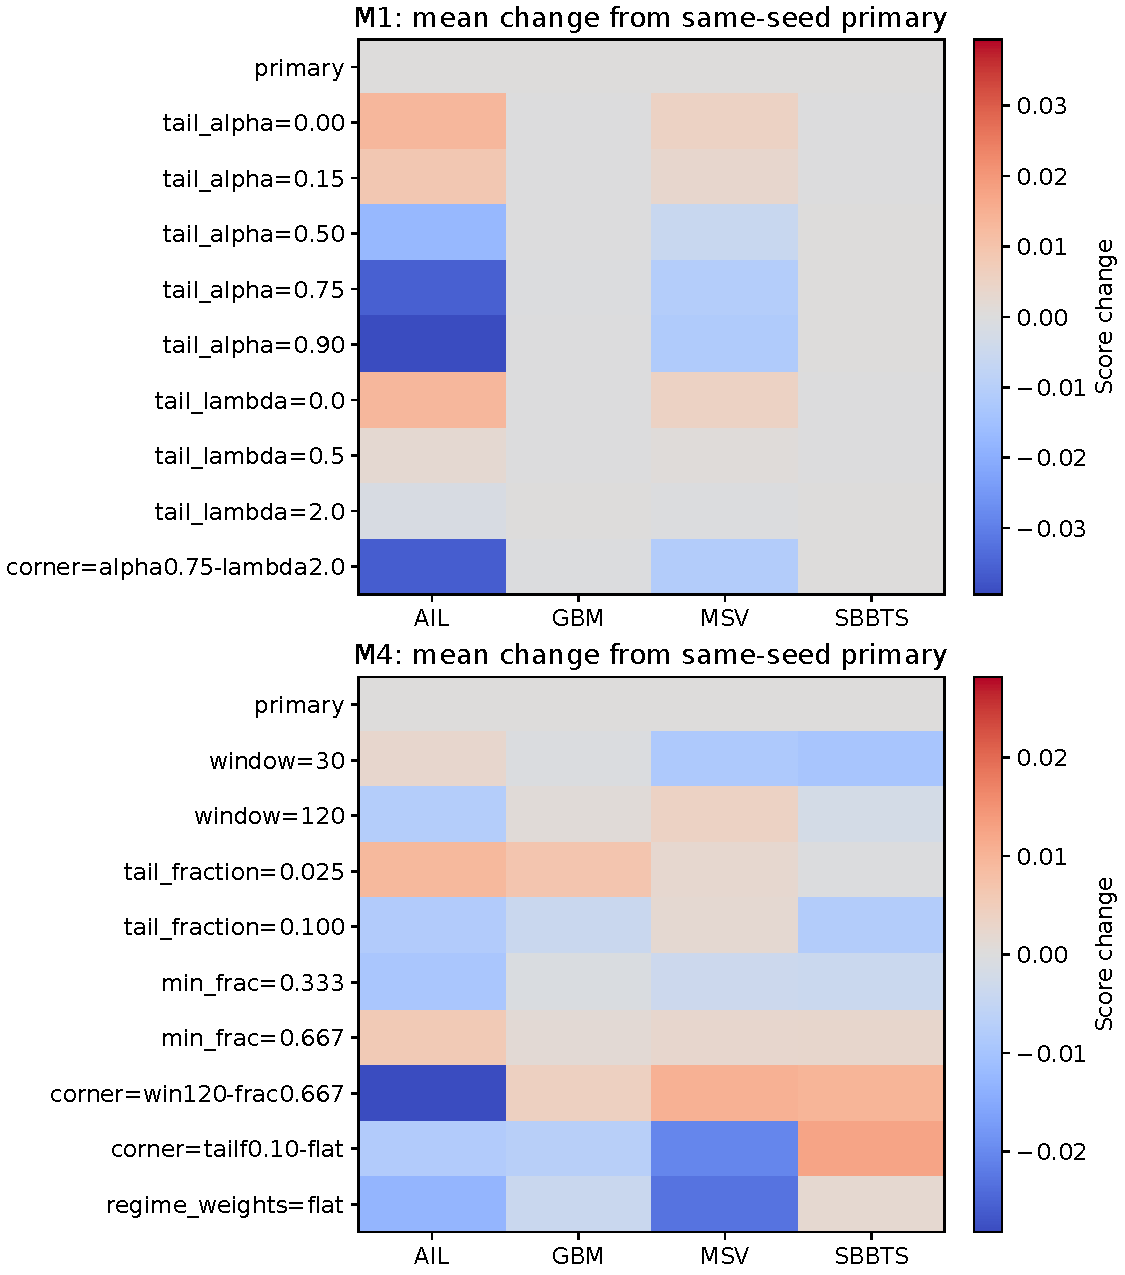
\includegraphics[width=\textwidth]{figures/sensitivity_scores.pdf}
\caption{\edited{Mean change in M1 and M4 scores from the same-seed primary,
over five seeds. Each panel shows the primary and the nine alternatives
affecting that metric; fixed M2 and M3 settings are omitted.}}
\label{fig:sensitivity-scores}
\end{figure}
\begin{figure}[htbp]
\centering
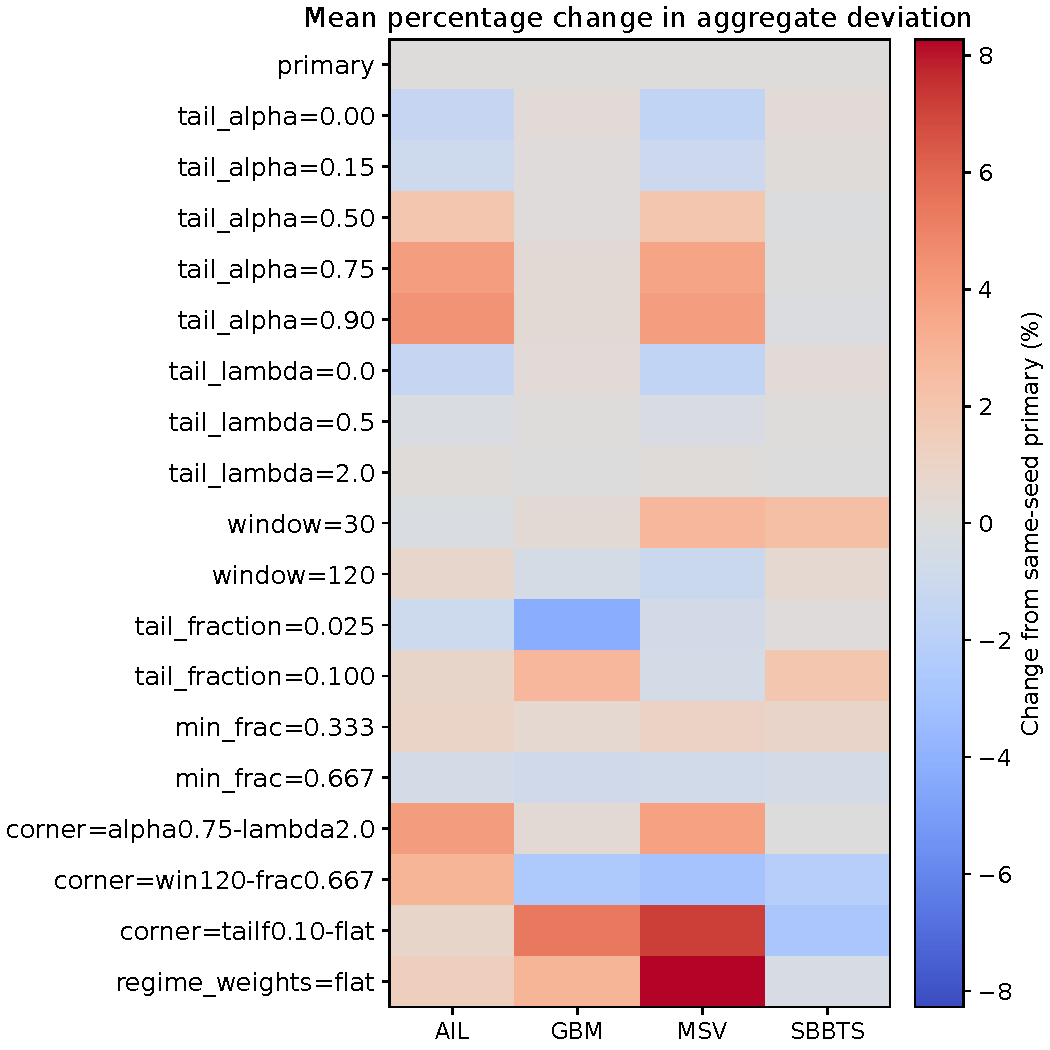
\includegraphics[width=\textwidth]{figures/sensitivity_aggregate.pdf}
\caption{\edited{Mean percentage change in aggregate deviation from the
same-seed primary. Lower aggregate deviation indicates closer gap parity.}}
\label{fig:sensitivity-aggregate}
\end{figure}
